% !TEX root = ../../../Lazcorreta.Tesis.tex
% \ABIERTO%

Otra de nuestras propuestas consistió en crear un fichero similar a \D en el que sustituimos las \transacciones originales por el conjunto de \ars que satisface cada una de ellas. La idea original era aplicar \apriori a este nuevo conjunto, \R, para analizar a través de las reglas que cumple cada transacción "`cómo"' se comportan los usuarios que las generan en lugar de estudiar "`qué"' ítems relacionan los usuarios en una transacción.

\subsubsection{Reescribiendo \D para obtener \R}
Para estudiar el comportamiento de un usuario es preferible analizar qué reglas "`verifica"' en vez de centrar el análisis en los ítems que forman dichas regla. Supongamos que un usuario visita los lunes un \portalWeb solicitando las páginas $A$, $B$ y $C$ y un conjunto de páginas $P_1$. Los viernes este usuario visita las páginas $A$, $G$ y $H$ y un conjunto de páginas $P_2$. Supongamos también que las páginas de $P_1$ y $P_2$ no están relacionadas frecuentemente con la página $A$ y que nuestro sistema de recomendación no considera variables temporales por lo que no puede determinar si es lunes o viernes. Cuando el usuario entra en el \portalWeb y solicita la página $A$ es muy probable que le recomendemos visitar la página $B$ o $G$ si estamos usando los métodos tradicionales de recomendación. Si el usuario visita a continuación $G$ el sistema recomendará la página $H$, a continuación alguna de las páginas de $P_2$ y por último la página $B$ con menor probabilidad. De cualquier modo el hecho de que visite la página $A$ no es tan significativo como la posibilidad de usar las reglas de comportamiento ya guardadas en nuestro sistema (las reglas que contienen la relación entre los \kitemsets $AGH$ y $P_2$). Nuestro objetivo es aprovechar la capacidad que tenemos de analizar las reglas que se verifican en nuestro \portalWeb de forma independiente al número de páginas que contienen, proporcionar un método para medir la relación existente entre las reglas de comportamiento de nuestro \portalWeb y usando únicamente las transacciones proporcionadas por los usuarios.

Si estudiamos las reglas verificadas por cada transacción del \dataset original \D, podemos definir el conjunto de reglas \R que contiene una línea por cada transacción de \D conteniendo las reglas que verifica la transacción original. El objetivo de esta conversión, $\D\hookrightarrow\R$, es analizar en un segundo estudio las reglas que contiene \R utilizando el algoritmo \apriori.

Inicialmente esta tarea es simplemente exploratoria y se necesitan muchas horas para convertir el \dataset original \D en grandes \datasets \R con diferentes umbrales de \soporte y confianza. Los \datasets de reglas tienden a ser mucho más grandes que los de transacciones. Si una transacción verifica una regla que contiene un determinado \kitemset $l_k$ también verificará todas las reglas de los \itemsets contenidos en $l_k$. Por ejemplo, si la transacción $ABCD$ genera una regla también generará las cincuenta reglas que se deducen de sus subconjuntos:
\begin{itemize}
  \item 14 reglas de 4 ítems: $ABC\rightarrow D$, $ABD\rightarrow C$, \ldots $D\rightarrow ABC$
  \item 24 reglas de 3 ítems: $AB\rightarrow C$, $AB\rightarrow D$, \ldots $D\rightarrow BC$
  \item 12 reglas de 2 ítems: $A\rightarrow B$, $A\rightarrow C$ \ldots $D\rightarrow C$
\end{itemize}

Si usamos un umbral de confianza bajo, una transacción de \D con dos ítems generará una línea con 2 reglas en \R, una transacción con 3 ítems generará 12 reglas, una transacción con 4 ítems generará 50 reglas. \R crecerá exponencialmente en función de la longitud de las transacciones de \D.

El desmesurado tamaño de los \datasets \R obtenidos nos condujo a hacer un análisis exploratorio de las diferencias existentes entre \R y \D con el fin de reducir los datos que forman \R sin perder la información que contiene.




\subsubsection{Análisis descriptivo de las diferencias existentes entre \D y \R}
En la sección TAL se expuso una modificación del algoritmo de generación de reglas con la que se puede trabajar con umbrales de confianza muy pequeños. La razón por la que buscamos esta reducción, que en algunos casos consistía en la eliminación del umbral, se entiende mejor al revisar los resultados obtenidos, que se muestran en la figura~\ref{fig:2-1-DvsR} y el cuadro~\ref{tab:2-2-2-DvsR}. Conforme se reduce el valor de \confianza mínima se pierde información de las transacciones en estudio. Por ejemplo, al usar un \soporte mínimo del 5\% en el \dataset \texttt{T40I10D100K} las reglas obtenidas se derivan únicamente de un 32.6\% de las transacciones del \dataset, de lo que se deduce que más del 67\% de las transacciones originales son completamente ignoradas por el análisis.

%\afterpage{\clearpage}
\begin{figure}[htb]
   \centering
   \begin{subfigure}[b]{0.44\textwidth}
      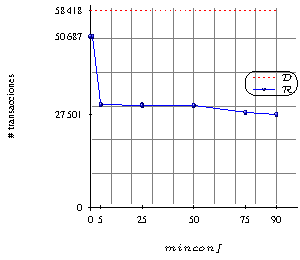
\includegraphics[width=\textwidth]{2-2-DvsR-foodmart-0_005.pdf}
      \caption{foodmart 0.005\%}
      \label{fig:2-1-foodmart0_005}
   \end{subfigure}%
   \hfill    
   \begin{subfigure}[b]{0.44\textwidth}
      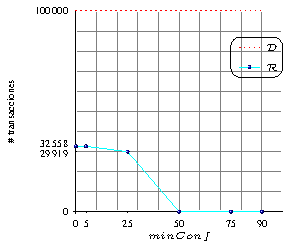
\includegraphics[width=\textwidth]{2-2-DvsR-T40I10D100K-5.pdf}
      \caption{T40I10D100K 5\%}
      \label{fig:2-1-T40I10D100K-5}
   \end{subfigure}
   \hfill
   \begin{subfigure}[b]{0.44\textwidth}
      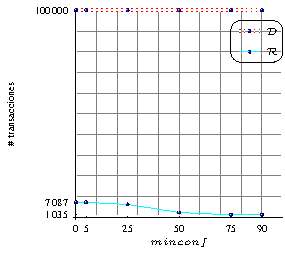
\includegraphics[width=\textwidth]{2-2-DvsR-T10I4D100K-1.pdf}
      \caption{T10I4D100K 1\%}
      \label{fig:2-1-T10I4D100K-1}
   \end{subfigure}
   \hfill    
   \begin{subfigure}[b]{0.44\textwidth}
      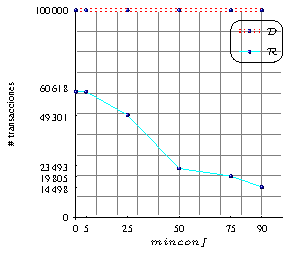
\includegraphics[width=\textwidth]{2-2-DvsR-T10I4D100K-0_5.pdf}
      \caption{T10I4D100K 0.5\%}
      \label{fig:2-1-T10I4D100K-0_5}
   \end{subfigure}
   \caption{\D vs \R}
\label{fig:2-1-DvsR}
\end{figure}

% \noindent
% \begin{table}[htb]
{\scriptsize
\begin{longtable}{cccccc}
   \caption{\D vs \R}\\
               &          &           & \multicolumn{2}{c}{transacciones} &            \\
   \hline
   fichero     & $minSup$ & $minConf$ &     \D      &        $\mathcal{R}$         & \D \'util \\ 
   \hline
\endfirsthead
   \multicolumn{6}{c}%
      {\tablename\ \thetable\ -- \textit{\ldots continuación}} \\
   \hline
               &          &           & \multicolumn{2}{c}{transacciones} &            \\ \cline{4-5}
   fichero     & $minSup$ & $minConf$ &     \D      &        $\mathcal{R}$         & \D \'util \\ 
   \hline
\endhead
\hline
\multicolumn{2}{r}{\textit{Continúa en la página siguiente\ldots}} \\
\endfoot
\hline
\endlastfoot
\centering
  foodmart & 0.005\% & 90\% & 58\,418  & 27\,501 & 47.1\% \\
           &         & 75\% &          & 28\,125 & 48.1\% \\
           &         & 50\% &          & 30\,201 & 51.7\% \\
           &         & 25\% &          & 30\,212 & 51.7\% \\
           &         & 5\%  &          & 30\,440 & 52.1\% \\
           &         & 1\%  &          & 50\,687 & 86.8\% \\
           &         & 0\%  &          & 50\,687 & 86.8.\% \\
   \hline
  T40I10D100K & 5\% & 50\% & 100\,000  & 0       & 0\%     \\         %Comprobado
				  &     & 25\% &           & 29\,919 & 29.9\%  \\         %Comprobado
              &     &  5\% &           & 32\,558 & 32.6\%  \\         %Comprobado
              &     &  0\% &           & 32\,558 & 32.6\%  \\         %Comprobado
              & 1\% & 50\% &           & 92\,227 & 92.2\%  \\         %Comprobado
				  &     & 25\% &           & 99\,956 & 100.0\% \\         %Comprobado
				  &     &  5\% &           & 99\,956 & 100.0\% \\
				  &     &  1\% &           & 99\,956 & 100.0\% \\
				  &     &  0\% &           & 99\,956 & 100.0\% \\
				      & 0.5\% &  50\% &        & 99\,835 & 99.8\% \\          %Comprobado
              % &     & 25\% &           & \, & \% \\
              % &     &  5\% &           & \, & .\% \\
              % &     &  1\% &           & \, & .\% \\
              % &     &  0\% &        & \, & .\% \\
              % & 0.1\% &  50\% &        & \, & .\% \\
              % &     & 25\% &           & \, & .\% \\
              % &     &  5\% &           & \, & .\% \\
              % &     &  1\% &           & \, & .\% \\
              % &     &  0\% &        & \, & .\% \\
   \hline
  T10I4D100K & 5\%   & 50\%  & 100\,000  & 0       & 0\%    \\
	           &       & 25\%  &           & 15\,475 & 15.5\% \\
             &       & 5\%   &           & 32\,558 & 32.6\% \\
             & 1\%   & 50\%  &           &  2\,211 &  2.2\% \\
			       &       & 25\%  &           &  6\,109 &  6.1\% \\
				     &       &  5\%  &           &  7\,087 &  7.1\% \\
				     &       &  1\%  &           &  7\,087 &  7.1\% \\
				     &       &  0\%  &           &  7\,087 &  7.1\% \\
				     & 0.5\% &  50\% &           & 23\,493 & 23.5\% \\
				     &       & 25\%  &           & 49\,301 & 49.3\% \\       %Comprobado
				     &       &  5\%  &           & 60\,618 & 60.6\% \\
				     &       &  1\%  &           & 60\,618 & 60.6\% \\
				     &       &  0\%  &           & 60\,618 & 60.6\% \\
             % & 0.1\% &  50\% &        & \, & .\% \\
             % &     & 25\% &           & \, & .\% \\
             % &     &  5\% &           & \, & .\% \\
             % &     &  1\% &           & \, & .\% \\
             % &     &  0\% &        & \, & .\%
\label{tab:2-2-2-DvsR}
\end{longtable}
}


Existen muchas aproximaciones en el estado del arte que buscan la reducción de las dimensiones del problema a tratar utilizando técnicas estadísticas basadas en la frecuencia de los ítems, sin embargo no se tienen en cuenta ciertos detalles, como el hecho de que los resultados son sólo significativos para un reducido grupo de individuos de la población en estudio.

En este trabajo usamos valores para el \soporte y \confianza mínimos que puedan ser utilizados en ordenadores personales convencionales sin generar problemas de falta de recursos, de modo que podamos atender al mayor número de individuos de la población en estudio. El tamaño de los \datasets \R obtenidos con estos parámetros es tan grande que no podemos analizarlos directamente por lo que proponemos un nuevo algoritmo para dividir \R en diferentes \datasets que puedan ser analizados convenientemente.



\subsubsection{División automática del \dataset de reglas}
Existen muchas investigaciones proponiendo métodos para dividir los \datasets originales de transacciones, pero todos ellos se basan en un alto control y \clasificacion del conjunto de ítems disponibles en el sistema. Nuestra propuesta no usa esta información adicional porque se obtiene de una gestión del sistema y no de del propio uso del mismo. Definimos un conjunto de familias de reglas para dividir el \dataset \R y agrupar aquellas reglas que los usuarios relacionan entre sí cuando interactúan con el sistema. A continuación se describe el algoritmo que proponemos.

\begin{enumerate}
  \item Seleccionar la regla con mayor \soporte, en caso de empate seleccionar la regla con mayor confianza y en caso de empate seleccionar la regla que contenga más ítems.
  $$R_1 = max_i\{soporte(R_i)\} \wedge$$
  $$\left(confianza(R_1) = max_j\{confianza(R_j) | soporte(R_j) = soporte(R_1)\} \right)$$
  Esta regla será el elemento principal de la primera familia de reglas, $\mathcal{F}_1$.
  \item Dividir \R en subconjuntos de reglas. El primer \dataset, $\R_1$, contendrá todas las líneas de \R que tengan la regla $R_1$ y el segundo \dataset, $\R_\infty$, contendrá el resto de líneas de \R.
  \item Ejecutar el algoritmo \apriori sobre $\R_1$ y aplicar de nuevo el paso 1 para seleccionar $R_2$, la regla de $\R_1$ que aparece con mayor frecuencia junto a $R_1$.
  \item Comprobar el \soporte de $R_2$ en $\R_\infty$: si el \soporte de $R_2$ en $\R_1$ es mayor que su \soporte en $\R_\infty$ se añade $R_2$ a la familia $\mathcal{F}_1$; en otro caso se elimina $R_2$ de $\R_1$.
  \item Volver al paso (3) mientras queden reglas no clasificadas en $\R_1$.
\end{enumerate}

Cuando se ha completado la definición de la primera familia de reglas se eliminan todas las reglas pertenecientes a $\mathcal{F}_1$ del \dataset original de reglas, \R, y las transacciones que queden vacías. A continuación se utiliza el mismo procedimiento para generar $\mathcal{F}_2$, la segunda familia de reglas. El algoritmo finaliza cuando $\R_\infty$ no contiene reglas asociadas, es decir, cuando todas las transacciones de $\R_\infty$ contienen únicamente una regla.



\subsubsection{Propuesta de sistema de recomendación}
Hemos definido un \sr en el que aplicar la modificación en dos pasos del algoritmo \apriori. El objetivo principal es obtener recomendaciones personalizadas para los usuarios de nuestro portal de educación, generando recomendaciones en tiempo real en forma de enlaces. El proceso se define a continuación:

\begin{enumerate}
  \item Un usuario entra en el sistema y selecciona el ítem $A$.
  \item El sistema sólo puede usar la información almacenada sobre los ítems directamente relacionados con $A$, es decir, las reglas originales cuyo antecedente es $A$ -- esta es la recomendación clásica basada en \ARs. La primera recomendación se basa únicamente en fecuencias (el sistema recomendará los consecuentes de las reglas con mayor \confianza que tengan al ítem $A$ como antecedente).
  \item El usuario selecciona un segundo ítem, $B$.
  \item A partir de ahora podemos usar la nueva información que hemos recogido sobre el comportamiento de la población de usuarios, las reglas que verifican en su visita a nuestro \portalWeb. Obtenemos las reglas derivadas del \kitemset $l_k$ y buscamos la familia a la que pertenecen, $\mathcal{F}_i$.
  \begin{itemize}
    \item Si $\mathcal{F}_i$ contiene reglas derivadas de las reglas verificadas por el usuario en esta visita, entonces hay una \confianza del 100\% entre las reglas descubiertas y las reglas verificadas por el usuario. En este caso el sistema recomendará los ítems de las reglas descubiertas con mayor \soporte. A diferencia de los métodos clásicos, esta propuesta descubre reglas que no tienen los ítems visitados por el usuario como antecedentes; esto es importante ya que el análisis realizado ignora por completo el orden de selección de los ítems.
    \item Si $\mathcal{F}_i$ no contiene reglas derivadas se usarán las reglas con mayor \confianza (y mayor \soporte en caso de empate) en relación con las reglas verificadas por el usuario. Adicionalmente, para resolver el problema de encontrar recomendaciones basadas en el antecedente, es posible encontrar reglas con cualquier ítem seleccionado por el usuario. Esto no puede llevarse a cabo con el método clásico.
  \end{itemize}
  \item El usuario selecciona un tercer ítem, $C$.
  \item Repetimos el tercer paso buscando una o más familias que contengan las reglas derivadas del \kitemset $l_k = \{A,B,C\}$.
\end{enumerate}

Esta aproximación conduce a una nueva experiencia con nuestro sistema educacional. Los usuarios se pueden sentir más confortables en su interacción con el sistema ya que pueden llevar a cabo sus tareas más rápidamente cuando utilizan los enlaces recomendados por el sistema.